\documentclass{article}
\usepackage[round]{natbib}
 
\usepackage{graphicx}
\usepackage{authblk}
\usepackage{amsmath}
\usepackage{graphicx}
\usepackage[margin=0.85in]{geometry}
\usepackage{lineno}
\usepackage{float}
\usepackage{cleveref}
\usepackage{tabularx,ragged2e}
\usepackage{url}
\usepackage[utf8]{inputenc}

\newcommand{\source}[1]{\hfill Source: {#1}} %command definition for sources in figures

\title{Supplementary:\\ Evaluating statistical Nitrogen Dioxide models using air quality sensors on board a carrier bicycle}
\author{Meng Lu et al. }
\date{\today}

\begin{document}

\maketitle

\section{Algorithm details}



\subsection{Random Forest Algorithm}
Introduced by Breiman\citep{breiman2001random}, random forest is a tree-structured classifier. To predict a class, a random forest classifier takes in samples and adopts the mode of votes from all trees as its result. A tree grows on independently identically distribution random vectors deducted from the sample set. The growth is measured by the decreasing generalised error $e$ defined here:
\begin{align}
    e &= P_{\boldsymbol X, Y}(mg(\boldsymbol X, Y)<0)\\
    mg(\boldsymbol X, Y) &= E (I(h_{k}(\boldsymbol{X} = Y))) -\max_{j\neq Y}(E(I(h_{k}(\boldsymbol X= j)))
\end{align}
$mg(\cdot)$ denotes the marginal function, $h_k$ the $k-th$ tree, $I(\cdot)$ the indication function, $\boldsymbol X$ and $Y$ are correspondingly the predictor and the response variables. The marginal function $mg(\cdot)$returns the difference of average votes class between $Y$, the tree output, and the second most voted class in the tree. The generalised error $e$ is defined as the probability of having negative marginal value. A negative marginal value suggests the frequency of having similar number of votes between the most favoured class the the second most favoured class. Thus, smaller the generalised error, more confident of the candidate random forest classifier in predicting its classes. Based on the selection criteria $e$ above, useful trees are selected and forms a random forest.

\subsection{Xgboost Algorithm}
XGBoost is a scalable fast computing tree boosting method \citep{chen2016xgboost}. Its efficiency partly comes from the modified tree learning structure that handles both weighted and sparse data. Besides, the parallel computation setting also ensures efficiency. Moreover, in contrast to existent tree splitting methods, its approximate tree splitting method fastens the greedy enumeration process.
Unlike Random Forest that takes the mode of all trees' prediction as output, this tree ensemble model sums the result of individual trees as output. The set of trees are chosen by minimizing the objective function $L$:
\begin{align}
    L(\phi) =& \sum_{i}\iota(\hat y_{i}, y_{i}) + \sum_{k}\Omega(f_{k})\\
    \Omega(f_{k}) =& \gamma T + \frac{1}{2}\lambda||\omega||^2
\end{align}
As the loss function, $\iota(\cdot)$ computes the difference between prediction $\hat y_{i}$ and sample  $y_{i}$. As the penalty function, $\omega(\cdot)$ increases when the tree gets more complicated in structure.  $f_{k}$ here stands for one regression tree that takes in predictors. $T$ and $\omega$ represent the number of leaves and the leaf weights accordingly. The regulation term $\frac{1}{2}\lambda||\omega||^2$ reduces over-fitting risk. 

\subsection{Lasso Algorithm}
Let \(\beta\) be the target coefficient set of Lasso. \(i\) and \(j\) are the number of samples and the number of independent factors accordingly. The algorithm tries to minimize \(\sum_{i = 1}^N{ (y_i - \sum_j\beta_j x_{ij})^2}\). As a tool, \(\delta_i\) is the tuple that has the form of (\(\pm1, \pm1,\pm1...\pm1\)). Define \( E\) as the equality set of \(\delta_i\) that meets the equality constraint \(\delta_i^T\beta = t\). Lasso parameter \( \mathnormal{t} \) controls the degree of shrinkage. The same paper has described three methods for the solution of  \( \mathnormal{t} \): cross-validation, generalized cross-validation and analytical unbiased estimation of risk. The Lasso algorithm consists of two major steps:
\par
\[
\begin{aligned}
&(1)\quad E =\{i_0\} \quad \textrm{where}\quad \delta_{i_0}= \textrm{sign} (\beta^0)\textrm{,}\\
&(2)\quad \textrm{While}\quad \sum\ |\beta_j| > t\textrm{:}\quad\textrm{Add}\quad i \quad \textrm{to the set} \quad E \quad \textrm{where} \quad \delta_i = \textrm{sign}(\beta).\quad \textrm{Find} \quad\beta = \textrm{argmin}(\sum_{i = 1}^N{ (y_i - \sum_j\beta_j x_{ij})^2)}
\end{aligned}
\]


  \subsection{Global NO$_2$ model predictions}
%The openaq data is used for the global model predictions (see Lu et al. 2020). Three methods are evaluated in this study, namely xgboost, random forest, and Lasso. Based on hyperparameter setting recommendations provided by Lu et al (2020) We used 1000 trees for all the methods. The maximum tree depth for xgboost is set to 6 and learning rate set to 0.02. Other settings are the same as Lu2020. 
As the global model predictions are for entire year, we scale them to the same time-span as the cargo-bike measurements by multiplying the predictions to the ratio between the global model prediction and the LML measurements averaged over the timespan of the cargo-bike measurements (July 16 -19, 8 am - 11 am), which means after scaling, the mean of the xgboost, random forest, and Lasso predictions are also 23.25 ug/m3 if scaled using the Graafseweg station and 14.03 if scaled using the Ruyterstraat station.



\subsection{Global model predictions}
The mean of xgboost, random forest, and Lasso predictions over the area of Nijmegen (called predictions) are respectively 25.77, 22.38, and 26.54 (ug/m3). The Nijmegen predictions are shown in figure X. From the figures, the xgboost and random forest predictions reveal more details, they also obtained a higher prediction accuracy (see the global paper) compared to Lasso. Comparing the figure X with the predictors (supplement figure SF2), it can be observed that the predictions reveal primary road patterns. The paired Pearson correlation between three Nijmegen predictions in are: 0.8 for random forest vs. Lasso, 0.81 for random forest vs. xgboost, and 0.94 for Lasso vs. random forest.
\begin{figure}[h!]
    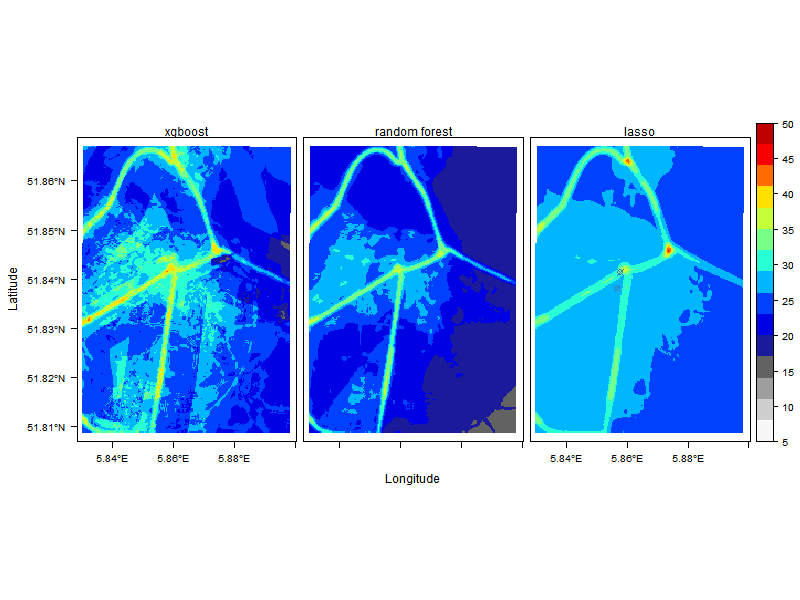
\includegraphics[width=\linewidth]{f3.png}
    \label{seperate}
    \caption {predictions from three global models: xgboost, random forest and lasso. The LML stations that are used in the global model are shown in the Lasso prediction plot.}
\end{figure}
\subsection{Validation with Cargo-bike measurements}

\begin{figure}[H]
    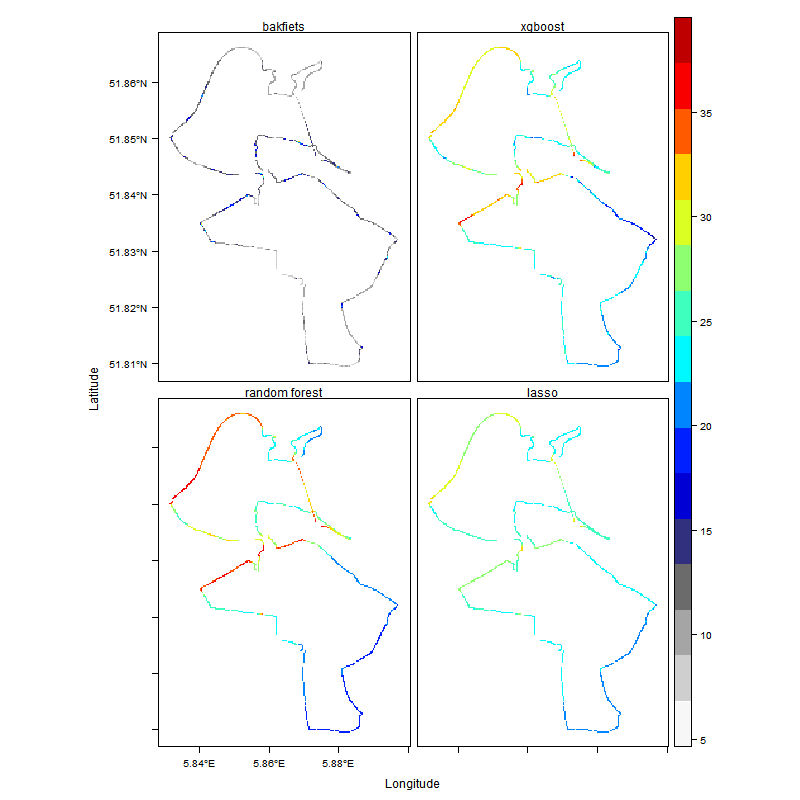
\includegraphics[width=\linewidth]{f4.png}
    \label{seperate}
    \caption {Averaged cargo-bike measurements and global model predictions (scaled). a: scale the cargo-bike using the Graafseweg LML station.}
\end{figure}
The cargo-bike measurements (the distribution is shown in supplementary figure SF1) show higher NO$_2$ in the west and middle, from points 19 -21, 24 -25, and around point 9 (figure 1, called route 19-21, 24-25, and 9), which align well with predictions from the three global models. However, the spatial variations of the cargo-bike measurements are much smaller compared to the global model predictions. The route 19-21 and route 24-25 are estimated much higher by the global models, most notably random forest.    
The global model predictions are higher in magnitudes, however, the mean of the global model prediction is closer to the mean of the LML ground station measurements. 
\begin{figure}[H]
    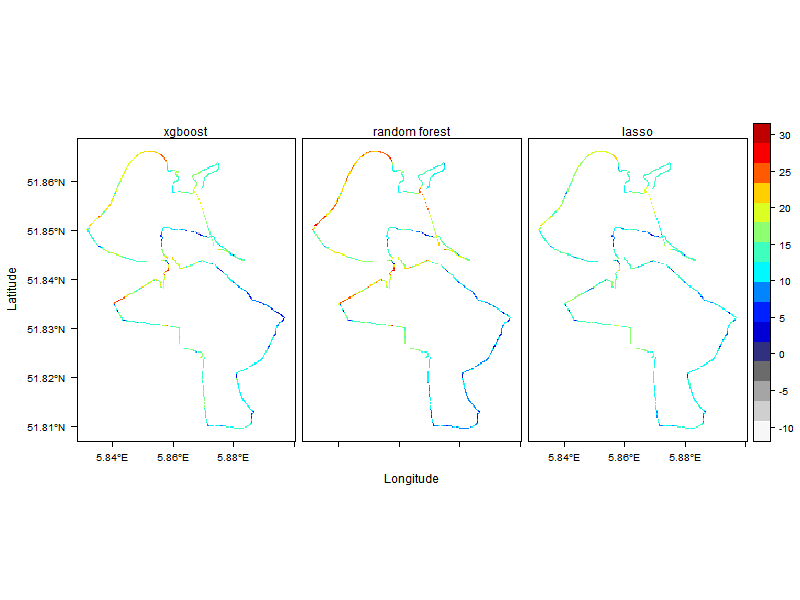
\includegraphics[width=\linewidth]{f4a.png}
    \label{Graafseweg}
    \caption {scale the cargo-bike using the Graafseweg station. The differences between scaled global model predictions and cargo-bike meausrements, the values are the subtraction of cargo-bike measurements from global model predictions (model prediction - bike measurements), in ug/m3.}
\end{figure}
\begin{figure}[H]
    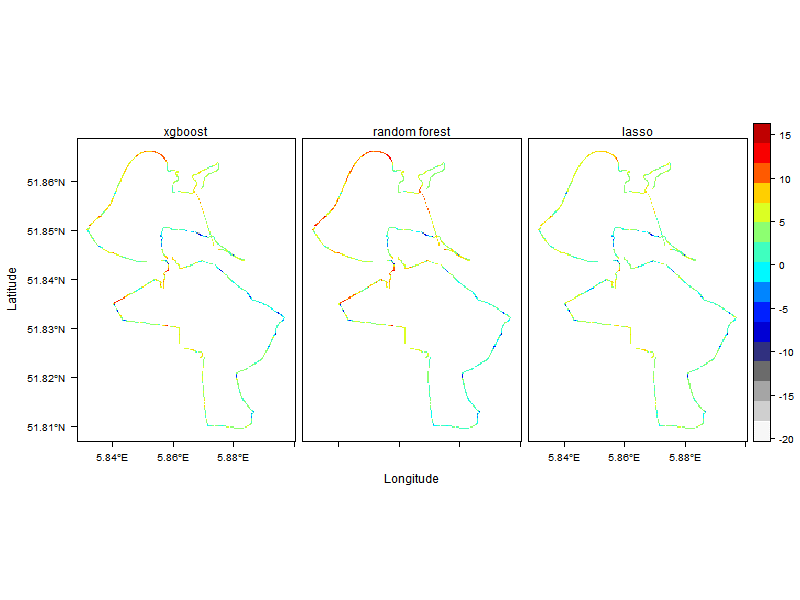
\includegraphics[width=\linewidth]{f4b.png}
    \label{ruyterstraat}
    \caption {scale the cargo-bike using the ruyterstraat station.}
\end{figure}

We make a distinction between the areas close to roads and far-away from roads. We define that if a location within 500 m distance away from the primary roads, it is considered as in traffic areas, else in background areas. \Cref{seperate} shows the cargo-bike routes that are in traffic and background areas.  
\begin{figure}[H]
    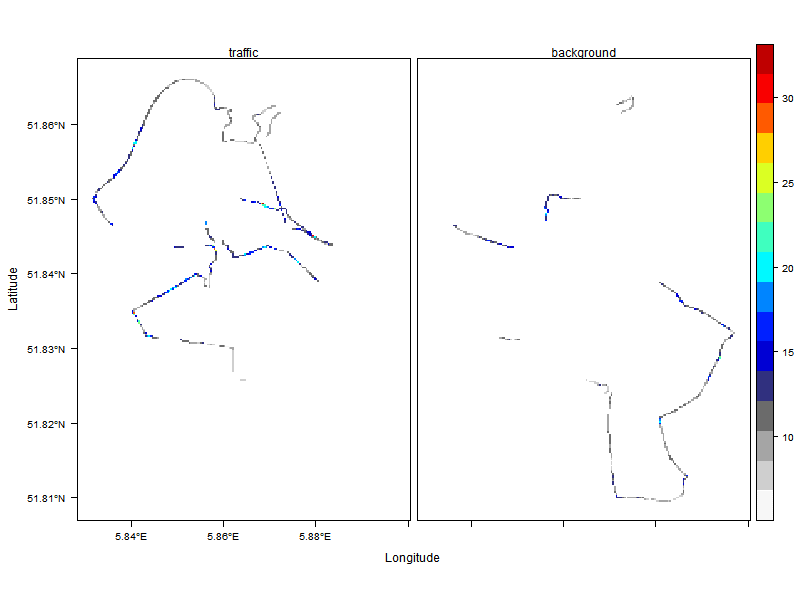
\includegraphics[width=\linewidth,trim=1cm 2cm 1cm 1cm, clip=true]{f2.png}
    \label{seperate}
    \caption {Cargo-bike route in traffic and background areas, .}
\end{figure}

\end{document}